\documentclass{ecnreport}

\stud{OD Robotique 2022-2023}
\topic{ROS 2 exam}

\begin{document}

\inserttitle{ROS 2 exam}

\insertsubtitle{2h, documents / internet allowed (closed chats please)}


\section{Description}

In this exam you will have to write a C++ node and run it two times through a launch file.\\

The package should first be compiled, then the simulation can be run once and for all with:
\begin{bashcodelarge}
 ros2 launch ecn_exam_2022 simulation_launch.py
\end{bashcodelarge}

This simulation involves the Baxter robot. The goal is to move the two arms by giving velocity commands on the end-effectors.\\

\subsection{Controlling the robot}

As in the labs, the simulation subscribes to:
\begin{itemize}
 \item \okt{/robot/limb/left/joint\_command}
 \item \okt{/robot/limb/right/joint\_command}
\end{itemize}
 on these topics, expected messages are of type \okt{baxter\_core\_msgs/msg/JointCommand}:
\begin{cppcode}
int32 mode        # control mode (should be set to VELOCITY_MODE here)
float64[] command # command (position or velocity)
string[] names    # names of the controlled joints

int32 POSITION_MODE =1
int32 VELOCITY_MODE =2
int32 TORQUE_MODE =3
int32 RAW_POSITION_MODE =4
\end{cppcode}

Depending on the arm that is controlled, the names of the joints are given below:
\begin{figure*}[h]\centering
 \raisebox{-.5\height}{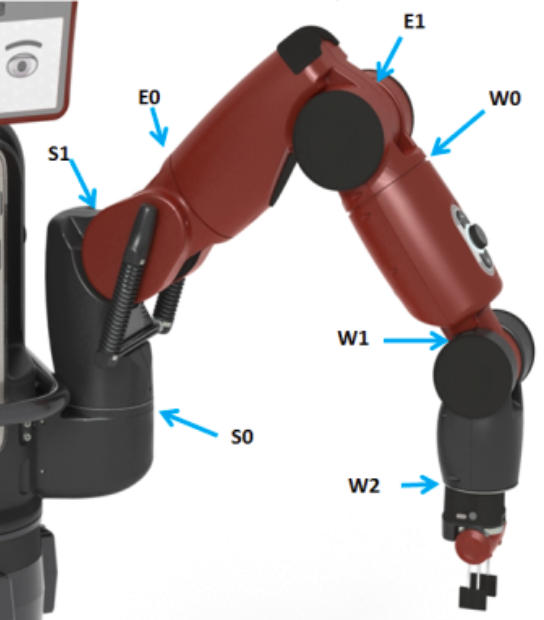
\includegraphics[width=.2\linewidth]{baxter}}\quad
  \begin{tabular}{|c|c|c|c|c|c|c|c|}
  \hline
  joints (\okt{left_} or \okt{right_})& \okt{s0} & \okt{s1}& \okt{e0} & \okt{e1} & \okt{w0} & \okt{w1} & \okt{w2} \\\hline
 \end{tabular}
\end{figure*}

\subsection{The Jacobian services}

Each arm advertizes a service to get the current Jacobian:
\begin{itemize}
 \item \okt{/robot/limb/left/jacobian}
 \item \okt{/robot/limb/right/jacobian}
\end{itemize}
These services are of type \okt{baxter\_simple\_sim/srv/Jacobian}:
\begin{cppcode}
float64[] position      # joint position to compute the Jacobian, current if empty
bool inverse false      # if the returned value should be the Jacobian inverse (true in our case)
bool ee_frame false     # if the Jacobian should be expressed in the end-effector frame (true in our case)
---
float64[42] jacobian   # the 42 coefficients of the Jacobian (or inverse) matrix, row-major
\end{cppcode}

\subsection{Publishing velocity setpoints}

Velocity setpoints can be published as \okt{geometry\_msgs/msg/Twist} through this launch file:
\begin{bashcodelarge}
 ros2 launch ecn_exam_2022 slider_launch.py
\end{bashcodelarge}

\section{Tips}

Compile the code once using \okt{colbuild --packages-select ecn_exam_2022}. Then, use \okt{gqt} in the package folder to configure QtCreator. Do not forget to use it with ROS 2 setup.\\

In order to efficiently debug your code, it is strongly advised to do the initial development with hard-coded values.
This node should do all necessary things with hard-coded parameters and topics.\\
You can then make it generic and run it through the launch file.\\

Feel free to have a look at the \okt{basic_node.cpp} from the lab templates.\\

Declaring node parameters is detailed in online tutorials and in my slides.\\

You can use the \okt{simple_launch} package to write the launch files.\\

 \newpage

\section{Writing the node}

The node is already more or less setup as \okt{control_node.cpp}. For now it does exactly nothing. The node should focus on one arm only.
It is strongly advized to program it for a given arm, then to make it generic.

The sampling time can be set to $dt = 0.1$ s.

The node should:
\begin{itemize}
 \item subscribe to velocity setpoints as published by the sliders
 \item publish to the joint command as subscribed by the simulation
 \item use a service call to the Jacobian to change a SE3 velocity setpoint to a joint velocity command
\end{itemize}
Note that in our case, the setpoint is given as the end-effector velocity twist, and we want to let the simulation compute the inverse for us. The two fields \okt{inverse} and \okt{ee\_frame} of the service request should be set to \okt{true}.

\subsection{Helper function to compute the command}

The \okt{eigen.h} header defines a helper function that will take care of computing the command:
\begin{cppcode}
std::vector<double> computeCommand(const JacobianInverseCoefs &Jinv_coeffs,
                                       const geometry_msgs::msg::Twist &v)
\end{cppcode}
This function boils down to applying the following computation:
\begin{equation*}
 \dot\q^* = \J^+\v
\end{equation*}

In practice, the function expects an array of 42 double (that is the \okt{jacobian} field of the response) and a \okt{Twist} that expresses the current setpoint.
It will return a \okt{std::vector<double>} of dimension 7, that corresponds to the joint velocity to apply on the robot.


\section{The launch file}

Once your node runs for a given arm, you should write a launch file that does the following for the left and right arms:
\begin{itemize}
 \item Run (include) the \okt{slider\_launch.py} in a proper namespace
 \item Run your node to control this arm with the slider
\end{itemize}



\end{document}
